\documentclass{beamer}
\beamertemplatenavigationsymbolsempty
\usetheme{Madrid}
\usepackage{graphicx, hyperref, amsmath, animate, tabularx, bm}
\usecolortheme{beaver}
\usefonttheme{professionalfonts}
\graphicspath{{./Figures/}}

\usepackage[backend=bibtex, style=verbose, sorting=none, autocite=footnote]{biblatex}
\addbibresource{References.bib}
\renewcommand*{\bibfont}{\scriptsize}
\setbeamerfont{footnote}{size=\tiny}

\title[DS 694: Seminar]{Cross-lingual Knowledge Transfer in Multi-lingual Language Models}
\author[Soumen Mondal]{Soumen Kumar Mondal\\\texttt{23m2157@iitb.ac.in}}
\institute[IIT Bombay]{Guide: Prof. Preethi Jyothi\\\;\\Indian Institute of Technology Bombay}
\date{May 8, 2024}

\begin{document}
	% Title page frame
	\begin{frame}
		\titlepage
	\end{frame}
	
	\begin{frame}{Introduction}
		\begin{block}{\scriptsize Problem Statement}\scriptsize
			\begin{itemize}
				\item \textbf{Objective:} 
				\begin{itemize}\scriptsize
					\item To explore and demonstrate the effectiveness of fine tuning methods in enhancing the adaptability and performance of multilingual language models across various languages and tasks.
					\item To develop methodologies that can improve the efficacy of factual knowledge transfer in multilingual setting.
				\end{itemize}				
				\item \textbf{Importance:} Multilingual models are essential for information exchange. Enhancing their efficiency and transferability without extensive retraining is important for practical usage.
			\end{itemize}
		\end{block}
		\begin{block}{\scriptsize Presentation Outline}\scriptsize
			\begin{itemize}
				\item \textbf{Language Model Fine Tuning:} Adapters, MAD-X, Composable SFT
				\item \textbf{Fact Representation:} Task Vectors, Cross Lingual Fact Representation
				\item \textbf{Geometry of Language Models:} Affine Language Subspaces
			\end{itemize}
		\end{block}
	\end{frame}
	
	\begin{frame}{Language Model Fine Tuning: Adapters}
		\begin{columns}
			\column{0.35\textwidth}
			\begin{block}{\scriptsize What is Adapter?}\scriptsize
				\begin{itemize}
					\item Adapters are small neural networks inserted between the layers of a pre-trained model.
					\item Each adapter only learns task-specific or language-specific features, leaving the original model weights untouched.
					\item This method is particularly advantageous for multilingual models because it enables the customization of a single foundational model for a variety of languages and tasks without the need for extensive retraining. 
				\end{itemize}		  
			\end{block}
			\column{0.55\textwidth}
			\begin{block}{\scriptsize Adapter Based Fine Tuning\footnotemark}
				\begin{figure}
					\centering
					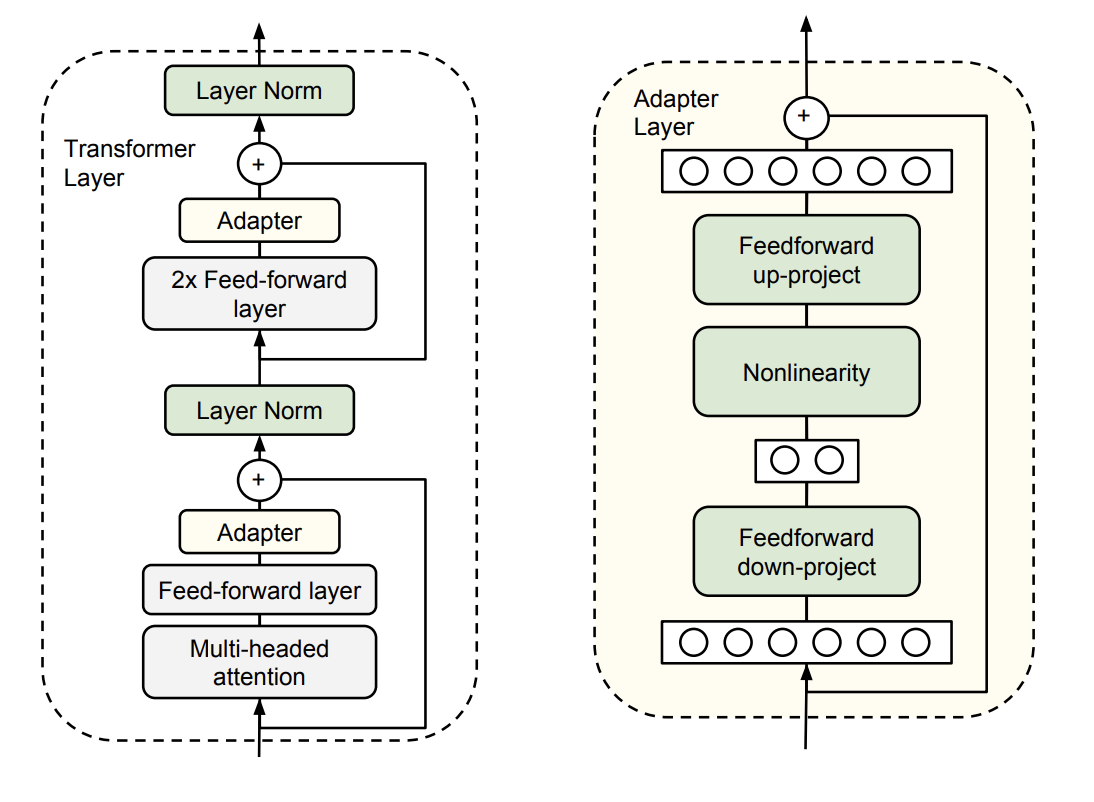
\includegraphics[width=\textwidth]{adapter}
				\end{figure}
			\end{block}
		\end{columns}\footcitetext{houlsby2019parameter}
	\end{frame}
	
	\begin{frame}{Language Model Fine Tuning: MAD-X}
		\begin{columns}
			\column{0.35\textwidth}
			\begin{block}{\scriptsize Overview of MAD-X}\scriptsize
				\begin{itemize}
					\item Language adapters are designed to adapt the model to the specificities of a given language. These adapters are trained using MLM on unlabelled data from the target language. 
					\item Task adapters are used to fine-tune the model for a specific task. They are applied after the language adapters
					\item The success of transfer learning heavily relies on the quality and comprehensiveness of the source language models.
				\end{itemize}		  
			\end{block}
			\column{0.55\textwidth}
			\begin{block}{\scriptsize MAD-X Architecture\footnotemark}
				\begin{figure}
					\centering
					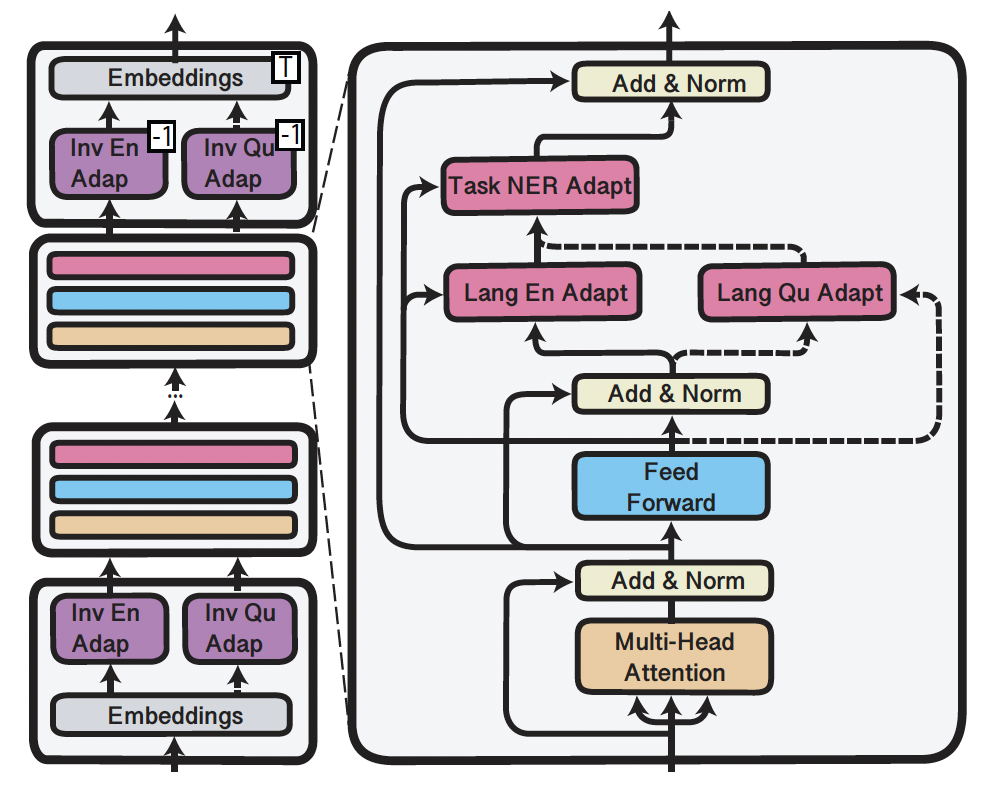
\includegraphics[width=\textwidth]{lang-task-adapter}
				\end{figure}
			\end{block}
		\end{columns}\footcitetext{pfeiffer2020mad}
	\end{frame}
	
	\begin{frame}{Language Model Fine Tuning: Composable SFT}
		\begin{block}{\scriptsize Overview of Composable SFT}\scriptsize
			\begin{itemize}
				\item Composable SFT selects a subset of parameters that exhibit significant changes during initial training and fine-tune only these parameters in subsequent phases as per the LTH.
				\item  Initially, the full model parameters $\theta^{(0)}$ are trained on target data, resulting in updated parameters $\theta^{(1)}$. 
				\item Parameters are reset to their original values $\theta^{(0)}$ and only those marked by $\mu$ (top $K$ based on absolute change) are updated in the subsequent training.
			\end{itemize}		  
		\end{block}
		\begin{columns}
			\column{0.35\textwidth}
			\begin{block}{\scriptsize Equations of SFT}\scriptsize
				The sparse fine-tuning can be represented as $ \phi = \theta^{(2)} - \theta^{(0)}$. Where $\theta^{(2)}$ are the parameters after sparse fine-tuning. The adaptation for a language and task can then be expressed as a function of the base model $F(\cdot; \theta + \phi_L + \phi_T)$.
			\end{block}
			\column{0.6\textwidth}
			\begin{block}{\scriptsize Composable SFT Process\footnotemark}
				\begin{figure}
					\centering
					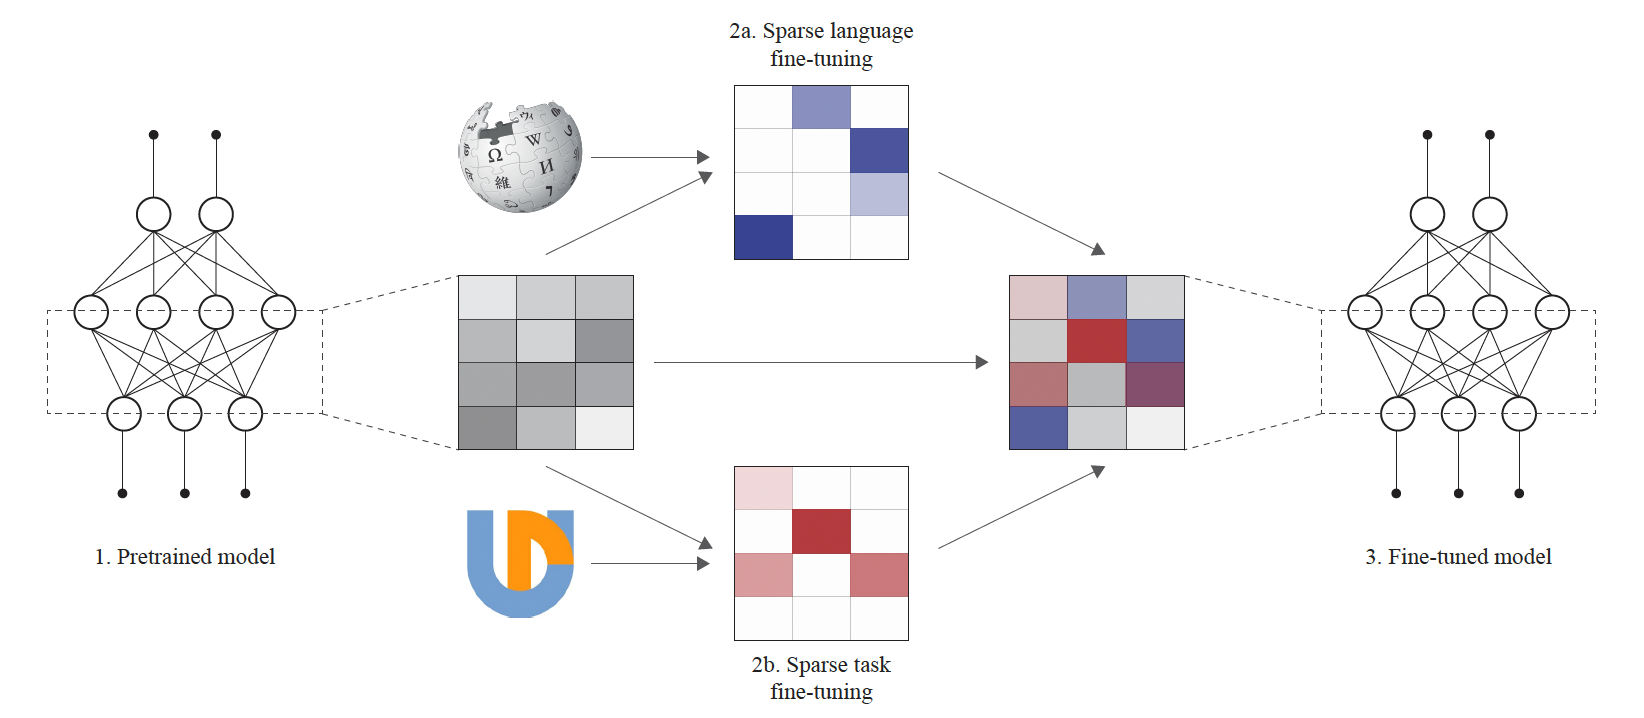
\includegraphics[width=\textwidth]{composable-sft}
				\end{figure}
			\end{block}
		\end{columns}\footcitetext{ansell2023composable}
	\end{frame}
	
	\begin{frame}{Fact Representation: Model Editing}
		\begin{block}{\scriptsize Overview of Task vectors}\scriptsize
			\begin{itemize}
				\item A task vector \( \tau_t \) is a vector that captures the changes made to a pre-trained model's weights when it is fine-tuned to perform a specific task ($\tau_t = \theta^t_{ft} - \theta_{pre}$)
				\item This vector \( \tau_t \) can be used to adjust the model weights of another pre-trained model of the same architecture to improve its performance on task \( t \), or combined with other task vectors or adjust the model's behavior such as unlearning a task.
				\item Task vectors involve element-wise operations on model weights, which assume a uniform structure across different model instances which could be a limitation.
			\end{itemize}
		\end{block}
		\begin{block}{\scriptsize Task Vectors in Model Editing\footnotemark}
			\begin{figure}
				\centering
				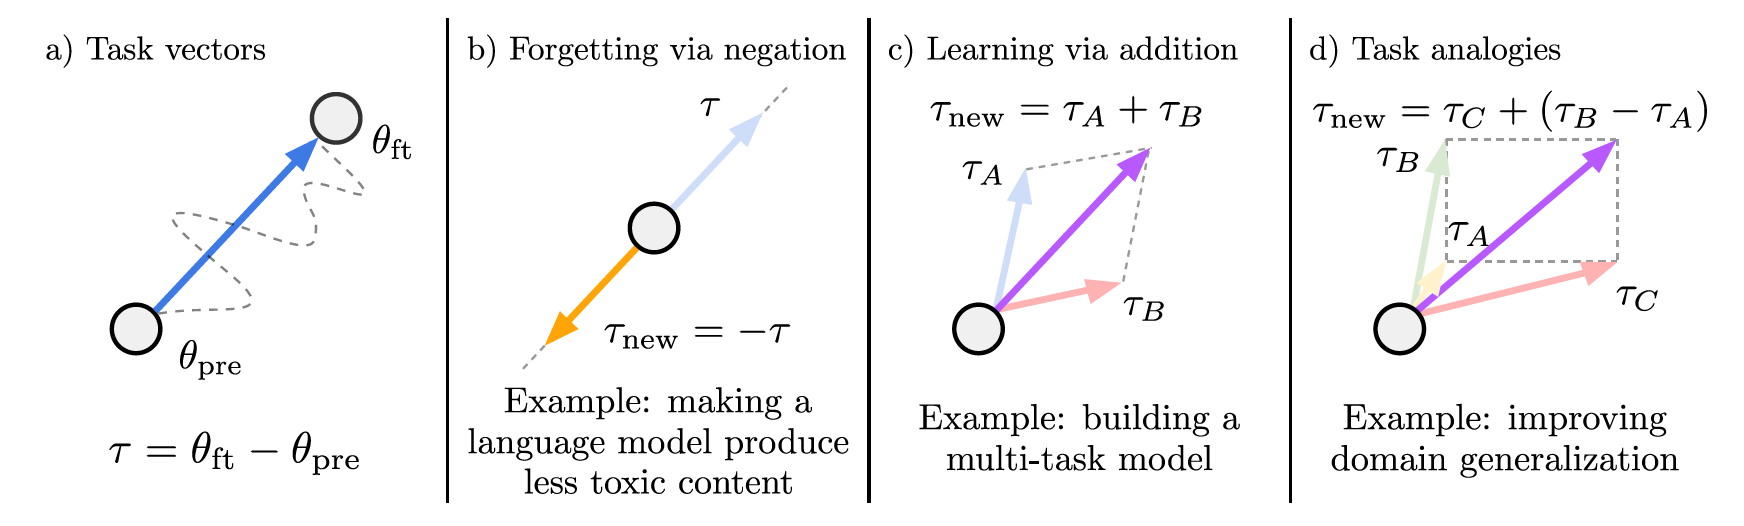
\includegraphics[width=0.75\textwidth]{task-vector}
			\end{figure}
		\end{block}\footcitetext{ilharco2023editing}
	\end{frame}
	
	\begin{frame}{Fact Representation: Cross Lingual}
		\begin{columns}
			\column{0.45\textwidth}
			\begin{block}{\scriptsize Overview of Fact Representation}\scriptsize
				\begin{itemize}
					\item \textbf{Language-Independent:} Each language has a unique set of neurons responsible for the representation of facts, independent of other languages.
					
					\item \textbf{Cross-Lingual Shared:} ML-LMs use the same set of neurons to represent the same facts across multiple languages. 
					
					\item \textbf{Cross-Lingual Transferred:} This representation type involves transferring factual knowledge from one language to others, typically from a high-resource language to low-resource languages.
				\end{itemize}
			\end{block}
			\column{0.45\textwidth}
			\begin{block}{\scriptsize Cross Lingual Fact Representation\footnotemark}
				\begin{figure}
					\centering
					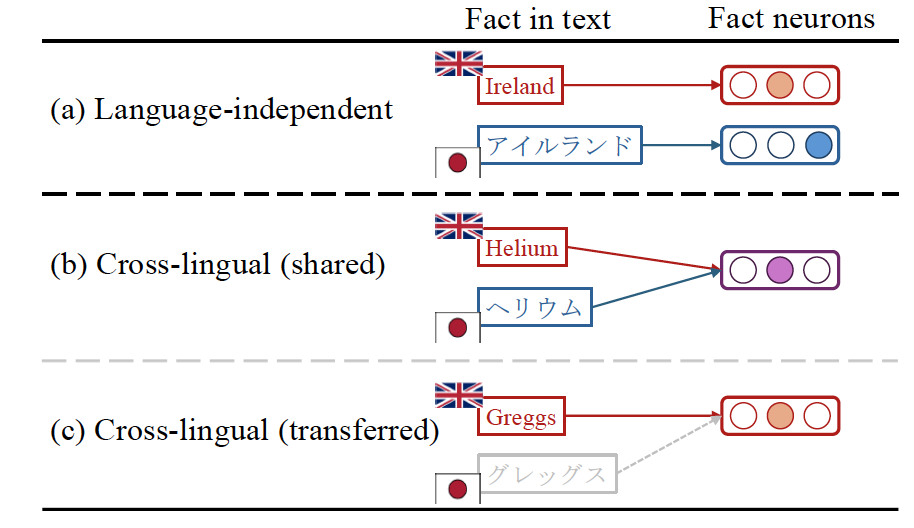
\includegraphics[width=\textwidth]{fact}
				\end{figure}
			\end{block}
		\end{columns}\footcitetext{zhao2024tracing}
	\end{frame}
	
	\begin{frame}{Fact Representation: Training Dataset}
		\begin{block}{\scriptsize Effect of Training Data Size}\scriptsize
			\begin{itemize}
				\item It has been found that the highest correlation (0.51) with probing accuracy (P@1) is observed for data-size of abstracts. 
				\item Italian and Japanese have P@1 score of 16.94\% and 1.34\% even though both of these languages are high resource with more than 100 MB of abstracts. 
				\item Afrikaans language despite being low resource (\textless 20 MB), shows high precision score (12.05\%) for factual probing.
			\end{itemize}
		\end{block}
		\begin{block}{\scriptsize Factual Probing Results\footnotemark}
			\begin{figure}
				\centering
				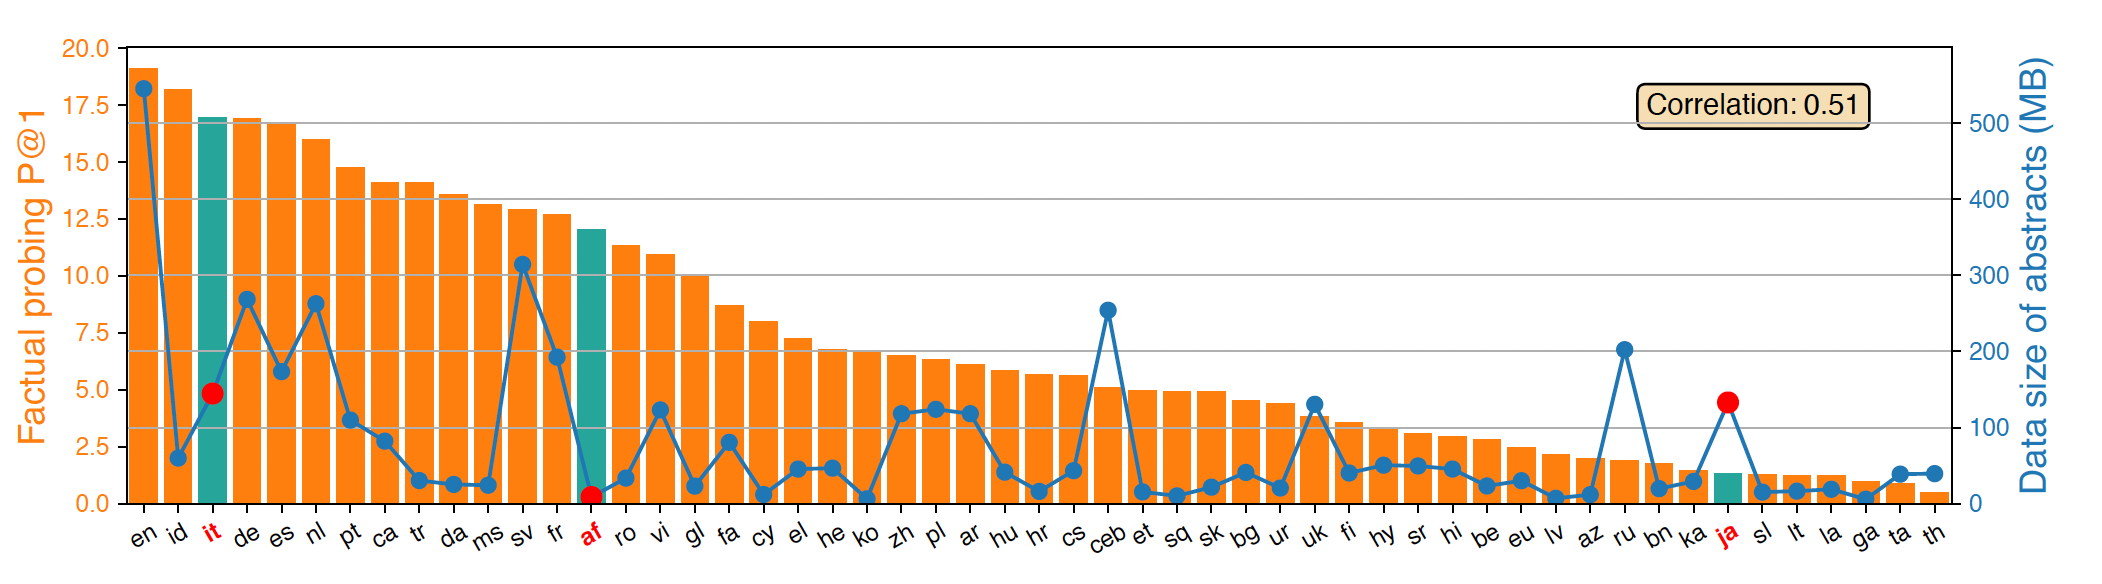
\includegraphics[width=0.85\textwidth]{data-volume}
			\end{figure}
		\end{block}\footcitetext{zhao2024tracing}
	\end{frame}
	
	\begin{frame}{Fact Representation: Tracing Roots}
		\begin{block}{\scriptsize Formation of Cross Lingual Fact Representation}\scriptsize
			\begin{itemize}
				\item To check if a given fact originates from the training data (Wikipedia), the roots is traced. If they co-occur, the fact is considered present, otherwise, it is considered as absent. 
				\item Many of the facts that were absent in the knowledge source but correctly predicted were relatively easy to predict because of entity tokens and naming cues.
				\item Facts in low resource languages are correctly predicted despite not being verifiable in the training corpus indicating a possibility of cross-lingual transfer.
			\end{itemize}
		\end{block}
		\begin{block}{\scriptsize Predicted Facts Results\footnotemark}
			\begin{figure}
				\centering
				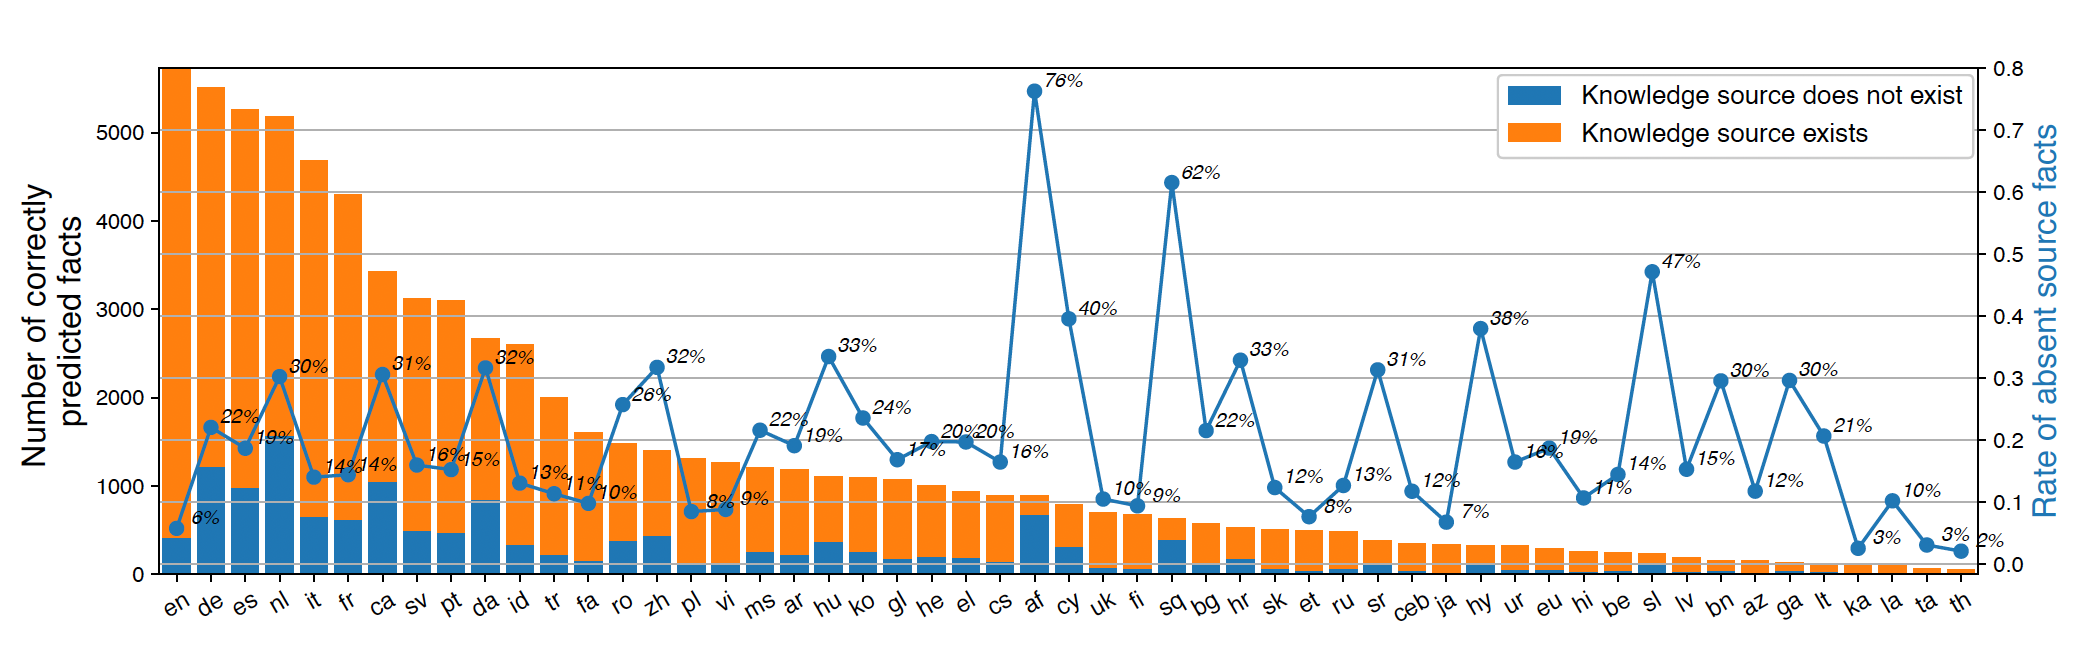
\includegraphics[width=0.7\textwidth]{pred-fact}
			\end{figure}
		\end{block}\footcitetext{zhao2024tracing}
	\end{frame}
	
	\begin{frame}{Geometry of Language Model Representation}
		\begin{block}{\scriptsize Affine Language Subspaces\footnotemark}\scriptsize
			\begin{itemize}
				\item The space contains embeddings or vectors assigned to tokens based on their semantic or syntactic properties. 
				\item Subspaces are low-dimensional vector space within the high-dimensional embedding space that capture certain linguistic properties. 
				\item The language sensitive axes are axes (basic vectors) that are within the subspace that capture language-specific information (e.g. grammar). 
				\item The language neutral axes are axes that are within the subspace encode information that is common across languages, such as word position or parts of speech.
				\item Languages tend to occupy similar linear subspaces in high-dimensional embedding spaces, after mean-centering.
			\end{itemize}
		\end{block}\footcitetext{chang2022geometry}
	\end{frame}
	
	\begin{frame}{Geometry of Language Model Representation}
		\begin{block}{\scriptsize Identification of Affine Language Subspaces}\scriptsize
			For a particular \emph{language A}, 512 input sentences are taken(each consists of 512 tokens) --- therefore giving a total 262K contextual tokens.
			\begin{equation}
				\mathbf{c}^{(i)} \in \mathbb{R}^d \text{ where } i \in \{1, 2, \dots , 262K\}
			\end{equation}
			\begin{equation}
				\bm{\mu}_A = \frac{1}{262K}\sum_{i=1}^{262K} \mathbf{c}^{(i)} \in \mathbb{R}^d \text{  ;  }
				S = \frac{1}{262K} \sum_{i = 1}^{262K} (\mathbf{c}^{(i)} - \bm{\mu}_A)(\mathbf{c}^{(i)} - \bm{\mu}_A)^T \in \mathbb{R}^{d \times d}
			\end{equation}
			After performing the eigenvalue decomposition on $S$, the top $k$ eigenvectors of $S$ are given by $V_A \in \mathbb{R}^{d \times k}$. The language subspace is identified by k eigenvector of $S$. $k$ is selected such that $q/p = 0.9$.
			\begin{equation}
				E = (\lambda_1, \lambda_2, \dots , \lambda_d) \text{ s.t. } \lambda_i \ge \lambda_{i+1} \quad \forall i \in \{1,2, \dots, d\} \text{    ;    }
				q = \sum_{i = 1}^{k} E[i] \text{    ;    }
				p = \sum_{i=1}^{d} E[i]
			\end{equation}
			
			The dimension of the context vector $d$ was originally 768 and if the value of reduced dimension $k$ is considered from each of the 12 layers of the transformer then the median value of $k$ was found to be 335.
		\end{block}
	\end{frame}
	
	\begin{frame}{Geometry of Language Model Representation}
		\begin{block}{\scriptsize Perplexity Ratio}\scriptsize
			The perplexity of the LLM is defined as:
			\begin{equation}\label{E:pp}
				pp(\mathbf{t}^{(i)}, \mathbf{t}^{(i-1)}, \dots , \mathbf{t}^{(1)}) = \prod_{i = 1}^{N} \left[ \frac{1}{\mathbb{P}(\mathbf{t}^{(i)} \mid \mathbf{t}^{(i-1)}, \dots , \mathbf{t}^{(1)})} \right]^{\frac{1}{N}}
			\end{equation}		
			\begin{equation}
				\mathbf{u} = V_A^T(\mathbf{x} - \bm{\mu}_A) \text{    ;    } \hat{\mathbf{x}} = V_A V_A^T (\mathbf{x} - \bm{\mu}_A) + \bm{\mu}_A
			\end{equation}
			\begin{equation}
				\text{Language-A:} \quad \mathbf{x}_A^{(i)[l]} \quad \forall i \in \{1, 2, \dots, N\},\; \forall l \in \{1, 2, \dots, 12\} \Longrightarrow pp_A^{[l]} 
			\end{equation}
			\begin{equation}
				\text{Language-A:} \quad \hat{\mathbf{x}}_A^{(i)[l]} = V_A^{[l]} V_A^{[l]^T} (\mathbf{x}_A^{(i)[l]} - \bm{\mu}_A^{[l]}) + \bm{\mu}_A^{[l]}  \quad \forall i, \; \forall l \Longrightarrow \hat{pp}_{A}^{[l]}
			\end{equation}
			\begin{equation}
				\text{Language-A:} \quad r_A^{[l]} = \frac{\hat{pp}_A^{[l]}}{pp_A^{[l]}} \quad \forall l \in \{0, 1, \dots , 12\}
			\end{equation}
			The average perplexity ratio over all the 88 languages for each of the layer is calculated as:
			\begin{equation}
				r^{[l]} = \frac{1}{88} \sum_{i = A}^{CJ} r_i^{[l]} \quad \forall l \in \{0, 1, \dots , 12\}
			\end{equation}
		\end{block}
	\end{frame}
	
	\begin{frame}{Geometry of Language Model Representation}
		\begin{columns}
			\column{0.6\textwidth}
			\begin{block}{\scriptsize Key Findings}\scriptsize
				\begin{itemize}
					\item Affine subspaces can be used for language modeling: To reconstruct the vectors of a particular \emph{language A} from its corresponding \emph{language subspace A}, the following equation can be used.
						\begin{equation}\label{E:Proj_A}
							Proj_A(\mathbf{x}_A) = V_A V_A^T (\mathbf{x}_A - \bm{\mu}_A) + \bm{\mu}_A 
						\end{equation}
					
					\item Language subspaces differed from one another: To reconstruct the vectors of a particular \emph{language A} from another \emph{language subspace B}, the following equation can be used.
						\begin{equation}\label{E:Proj_B}
							Proj_B(\mathbf{x}_A) = V_B V_B^T (\mathbf{x}_A - \bm{\mu}_B) + \bm{\mu}_B
						\end{equation}
						
					\item Mean-shifted subspaces were similar to one another: To reconstruct the vectors of a particular \emph{language A} after mean centering from another \emph{language subspace B}, the following equation can be used.
						\begin{equation}\label{E:Proj_B_mu_A}
							Proj_{B, \bm{\mu}_A}(\mathbf{x}_A) = V_B V_B^T (\mathbf{x}_A - \bm{\mu}_A) + \bm{\mu}_A
						\end{equation}
				\end{itemize}
			\end{block}
			\column{0.3\textwidth}
			\begin{block}{\scriptsize Results\footnotemark}\scriptsize
				\begin{figure}
					\centering
					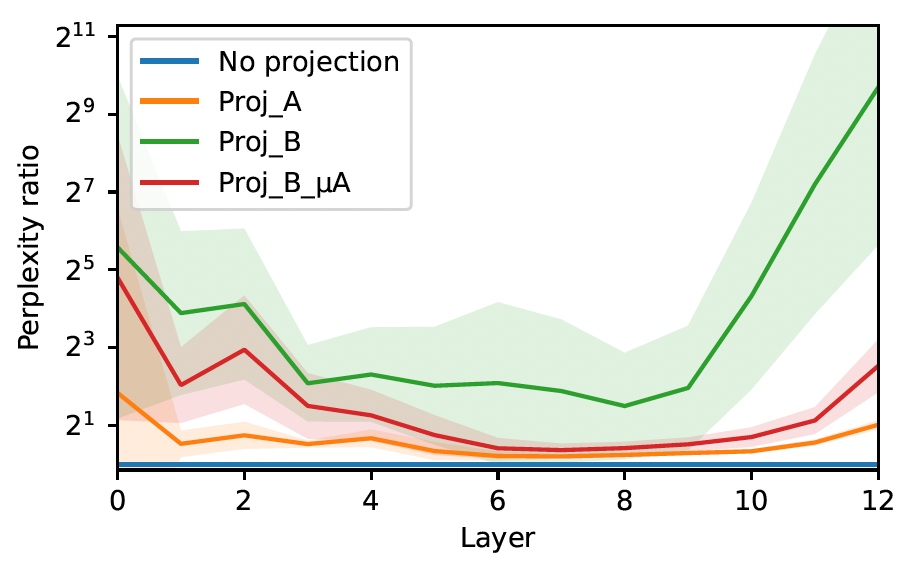
\includegraphics[width=\textwidth]{proj}
				\end{figure}
			\end{block}\footcitetext{chang2022geometry}
		\end{columns}
	\end{frame}
	
	\begin{frame}{Conclusion}
		\begin{block}{\scriptsize Summary}\scriptsize
			\begin{itemize}
				\item This study highlights the significance of language model fine-tuning techniques such as adapter-based fine-tuning and composable sparse fine-tuning.
				
				\item Moreover, the analysis of fact representation in language models highlight on the importance of task-specific model editing, cross-lingual fact representation, and the underlying geometry of language model representation. 
			\end{itemize}
		\end{block}
		\begin{block}{\scriptsize Future Directions}\scriptsize
			\begin{itemize}
				\item We can explore different versions of the Lottery Ticket algorithm to improve efficiency. Additionally, experimenting with other pruning methods like DiffPruning\footnotemark and ChildTuning\footnotemark could help refine our approach. 
				\item We can plan to improve how multilingual language models represent factual knowledge across languages. This includes developing better methods for cross-lingual fact representation learning and creating more accurate datasets for probing factual knowledge. 
			\end{itemize}
		\end{block}
		\footcitetext{guo2021parameterefficient}\\
		\footcitetext{xu2021raise}
	\end{frame}

	\section{References}
	\begin{frame}{References}
		\begin{block}{}\scriptsize
			\printbibliography
		\end{block}
	\end{frame}
	
	\begin{frame}{}
		\centering \Huge
		\emph{Thank You!}
	\end{frame}
	
\end{document}